\documentclass[12pt,a4paper]{article}
\usepackage[spanish,es-tabla]{babel}
\usepackage[utf8]{inputenc}
\usepackage{graphicx}
\usepackage{hyperref}
\usepackage{makecell}
\usepackage{float}
\usepackage{natbib}

\title{Proyecto}
\author{Gabriel Abellán Rodríguez}
\date{\today}

\begin{document}
\begin{titlepage}
    \centering
    
\includegraphics[width=0.4\textwidth]{images/LogoRiberaNuevo.png}\par
    \vspace{1cm}
    {\bfseries\LARGE I.E.S. Ribera del Tajo \par}
    \vspace{1cm}
    {\scshape\Large Técnico Superior en Administración de Sistemas Informáticos en Red
    \par}
    \vspace{3cm}
    {\scshape\Huge Tarea PIMAS 02 \par}
    \vspace{3cm}
    {\itshape\Large Proyecto intermodular de Administración de Sistemas Informáticos en Red \par}
    \vfill
    {\Large Autor:\par}
    {\Large Gabriel Abellán Rodríguez \par}
    \vfill
    {\Large \today \par}
\end{titlepage}

\tableofcontents
\newpage

\section{Introducción}

El presente proyecto tiene como objetivo fundamental el diseño, desarrollo e implementación de una plataforma web transaccional orientada a la comercialización e información de juegos de cartas coleccionables (JCC). Este sector ha experimentado un crecimiento sostenido en los últimos ejercicios, tanto en volumen de usuarios como en el consumo de productos asociados. La solución propuesta no solo constituye un entorno de comercio electrónico B2C (Business-to-Consumer) para la adquisición de productos y accesorios, sino que también actúa como un repositorio documental y formativo para usuarios de diversos niveles de experiencia.

La plataforma se estructura en módulos funcionales diferenciados: una tienda en línea para la comercialización de productos, un apartado de guías técnicas introductorias para los principales sistemas de juego del mercado, y una sección de divulgación normativa. Este enfoque centraliza servicios y conocimientos que habitualmente se encuentran fragmentados en la red.

A nivel de interfaz de usuario (UI) y experiencia de usuario (UX), el diseño se basa en principios de accesibilidad, usabilidad y diseño adaptativo (Responsive Web Design), garantizando la correcta visualización en dispositivos de escritorio y móviles. Adicionalmente, se ha implementado soporte multi-idioma (español e inglés) para facilitar la internacionalización del servicio.

El desarrollo de esta infraestructura tecnológica constituye la aplicación práctica de los conocimientos adquiridos durante el ciclo formativo de grado superior en Administración de Sistemas Informáticos en Red (ASIR). Esto abarca desde el despliegue de la capa de presentación (frontend) y lógica de negocio (backend), hasta el diseño de la persistencia de datos, la configuración de topologías de red seguras, la configuración de servidores y el establecimiento de políticas de alta disponibilidad.

\newpage
\section{Módulos Implicados}
\label{Modulos}

El desarrollo arquitectónico e implementación técnica del proyecto se fundamentan en las siguientes áreas de conocimiento:

\begin{itemize}
    \item \textbf{Administración de Sistemas Operativos:} Despliegue y configuración de entornos de servidor híbridos (Windows Server 2019/2022 y distribuciones GNU/Linux Ubuntu). Implementación de rutinas de copias de seguridad de la base de datos (Disaster Recovery).
    \item \textbf{Planificación y Administración de Redes:} Diseño de la topología lógica, segmentación mediante VLANs y configuración de reglas de enrutamiento y cortafuegos para aislar entornos críticos.
    \item \textbf{Fundamentos de Hardware:} Planificación de los requisitos físicos para la infraestructura de servidores virtuales y sistemas de almacenamiento.
    \item \textbf{Inglés:} Integración de funcionalidades de internacionalización en la plataforma, permitiendo la conmutación dinámica del contenido entre español e inglés.
    \item \textbf{Lenguaje de Marcas y Sistemas de Gestión de Información:} Construcción de la capa de presentación mediante HTML5 y CSS3, aplicando metodologías de diseño modular. Integración de interactividad asíncrona mediante JavaScript.
    \item \textbf{Implantación de Aplicaciones Web:} Configuración de servidores web (Internet Information Services - IIS) y despliegue del entorno de ejecución PHP en sistemas Windows para la lógica de negocio.
    \item \textbf{Gestión de Bases de Datos:} Diseño e implementación del esquema relacional en clústeres MariaDB Master-Master. Uso de replicación para garantizar la integridad referencial y automatizar la sincronización de datos.
    \item \textbf{Seguridad y Alta Disponibilidad:} Aplicación de políticas de bastionado (Hardening), despliegue de balanceadores de carga en capa 7 (HAProxy) y monitorización avanzada mediante Zabbix.
    \item \textbf{Itinerario Personal para la Empleabilidad:} Formulación del plan de Prevención de Riesgos Laborales (PRL) asociado al entorno tecnológico y logístico del proyecto.
\end{itemize}

\newpage
\section{Estudio de Mercado y Viabilidad Comercial}
\label{EstudioMercado}

\textbf{Público Objetivo:} El segmento de mercado principal comprende usuarios de entre 15 y 35 años, con perfiles orientados al coleccionismo y al juego competitivo de la franquicia Pokémon. La fase inicial de despliegue logístico se acotará al territorio nacional (España), con proyecciones de escalabilidad hacia el mercado europeo a medio plazo.

\textbf{Análisis de la Competencia:} El ecosistema de venta de JCC presenta una alta saturación. Para establecer una ventaja competitiva, la plataforma propuesta enfatiza una experiencia de usuario (UX) superior y tiempos de respuesta logísticos optimizados, garantizados por una infraestructura tolerante a fallos.

\textbf{Demanda:} El mercado de coleccionables mantiene una curva de demanda sostenida y alcista, impulsada por la nostalgia y el factor coleccionable de los activos.

\section{Análisis DAFO (Debilidades, Amenazas, Fortalezas y Oportunidades)}
\label{DAFO}

\textbf{Debilidades:}
\begin{itemize}
    \item Dependencia inicial en la gestión manual de operaciones logísticas.
    \item Posicionamiento nulo en la fase de lanzamiento (Start-up).
    \item Requerimiento de capital de trabajo elevado para el acopio inicial de inventario.
\end{itemize}

\textbf{Amenazas:}
\begin{itemize}
    \item Roturas de cadena de suministro por parte de los distribuidores.
    \item Fluctuaciones en las tarifas de los operadores logísticos.
\end{itemize}

\textbf{Fortalezas:}
\begin{itemize}
    \item Estructura de costes operativos fijos iniciales mínimos.
    \item Arquitectura web de grado empresarial (Alta disponibilidad, monitorización proactiva) que transmite confiabilidad y minimiza el tiempo de inactividad.
\end{itemize}

\textbf{Oportunidades:}
\begin{itemize}
    \item Expansión continua del mercado de coleccionables en Europa.
    \item Posibilidad de generar sinergias mediante contenido en redes sociales.
\end{itemize}

\newpage
\section{Catálogo de Servicios Digitales}
\label{Servicios}

\subsection{Comercio Electrónico B2C}
El servicio central consiste en una plataforma de e-commerce transaccional. La base de datos segmenta el catálogo en dos líneas principales: productos sellados y el mercado secundario de cartas sueltas.

\subsection{Gestión Logística}
Se ha implementado un flujo de gestión de pedidos integrado, diseñado para coordinar la expedición a través de operadores logísticos nacionales.

\subsection{Autenticación y Verificación de Identidad}
Se ha implementado un flujo de autenticación robusto, previniendo el alta de cuentas sintéticas y garantizando la trazabilidad de los usuarios en un entorno seguro.

\newpage
\section{Arquitectura de Persistencia de Datos}
La persistencia de información se soporta sobre un motor de bases de datos relacional (MariaDB), configurado en un entorno clústerizado para asegurar la replicación ininterrumpida de los catálogos y usuarios.

\subsection{Esquema Relacional}
El modelo de datos garantiza la integridad referencial y se apoya en restricciones para automatizar el control de concurrencia y los flujos de inventario entre los distintos servidores.

\begin{figure}[H]
    \centering
    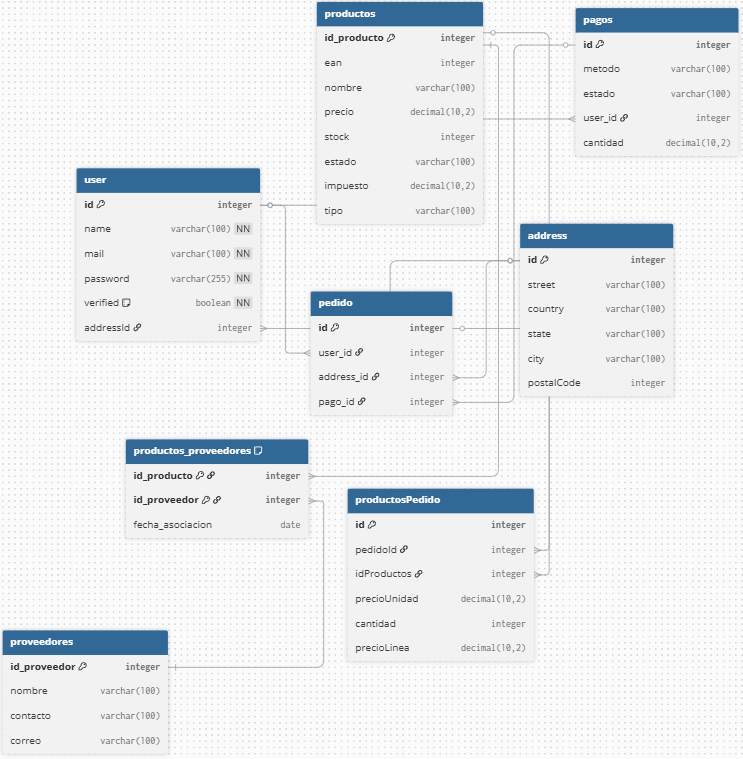
\includegraphics[width=0.8\linewidth]{images/dbdiagram.png}
    \caption{Diagrama Entidad-Relación de la base de datos.}
\end{figure}

\newpage
\section{Stack Tecnológico y Desarrollo Web}
\label{PaginaWeb}

La solución adopta una arquitectura de alta disponibilidad, segmentada en capas de presentación, lógica de negocio y persistencia distribuida.

\subsection{Definición del Stack}
\begin{itemize}
    \item \textbf{Capa de Presentación (Frontend):} Desarrollada en HTML5 semántico y CSS3 puro para garantizar un renderizado ligero.
    \item \textbf{Capa Lógica (Backend):} Procesamiento soportado por PHP sobre servidores Windows (IIS). Se han habilitado las extensiones \texttt{mysqli} y \texttt{pdo\_mysql} para optimizar la conexión con los nodos de datos.
    \item \textbf{Capa de Datos (SQL):} Desplegada sobre nodos Linux corriendo MariaDB en clúster, utilizando sentencias preparadas en PHP para garantizar la seguridad frente a inyecciones SQL.
\end{itemize}

\newpage
\section{Continuidad de Negocio: Backup y Recuperación (Disaster Recovery)}
\label{Backup}

La estrategia de respaldos se automatiza a nivel de sistema operativo mediante tareas programadas, encargadas de ejecutar volcados de la base de datos a intervalos regulares. Estos archivos resultantes son almacenados en repositorios aislados, posibilitando una restauración rápida en caso de contingencia.

\newpage
\section{Infraestructura y Segmentación de Red}
\label{RedInterna}

El diseño de la topología de red constituye el núcleo crítico del despliegue, fundamentándose en principios de defensa en profundidad y segmentación lógica para mitigar vectores de ataque.

\begin{figure}[H]
    \centering
    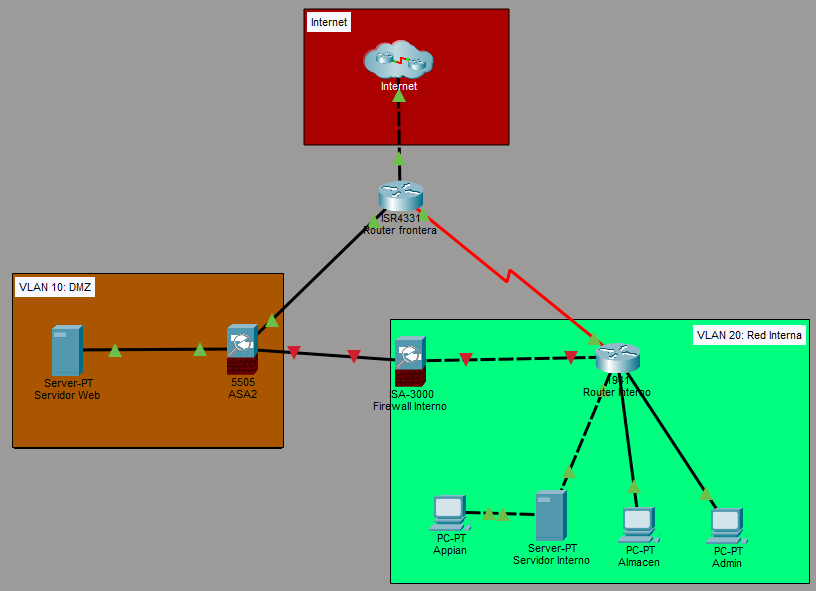
\includegraphics[width=0.9\linewidth]{images/esquemaRed.png}
    \caption{Topología de red y segmentación lógica mediante pfSense.}
\end{figure}

\subsection{Enrutamiento y Segmentación (VLANs)}
La red se administra mediante el cortafuegos perimetral \textbf{pfSense}, que actúa como gateway y gestor de tráfico entre las siguientes zonas:
\begin{itemize}
    \item \textbf{WAN (World Wide Web):} Interfaz con salida a la red pública.
    \item \textbf{Zona Desmilitarizada (DMZ - 192.168.10.0/24):} Aloja el balanceador HAProxy y los servidores web frontales IIS. Es el único segmento que procesa tráfico entrante filtrado desde el exterior.
    \item \textbf{Red Interna Protegida (LAN - 192.168.20.0/24):} Segmento estanco donde reside el clúster de bases de datos y la gestión de telemetría.
\end{itemize}

\newpage
\section{Memoria Técnica: Infraestructura de Alta Disponibilidad}
\label{AltaDisponibilidad}

Este proyecto implementa una arquitectura orientada a la continuidad de negocio, eliminando los Puntos Únicos de Fallo (SPOF) mediante redundancia en todas las capas.

\subsection{Capa Frontal y Balanceo de Carga (HAProxy)}
Se ha desplegado un servicio \textbf{HAProxy} operando en capa 7 (HTTP) dentro de la DMZ para gestionar la carga transaccional:
\begin{itemize}
    \item \textbf{Distribución de Carga:} Implementación del algoritmo \textit{Round Robin} para repartir el tráfico entrante de forma equitativa entre el pool de servidores web.
    \item \textbf{Health Checks (Sondeo de Salud):} Supervisión activa y constante del puerto 80 de los nodos web. Ante un fallo en el servicio IIS o caída del nodo, HAProxy ejecuta un \textit{failover} automático, retirando el nodo de la rotación y garantizando que la interrupción sea transparente para el usuario final.
\end{itemize}

\subsection{Capa de Aplicación (Windows Server / IIS)}
La lógica de negocio se procesa en una granja de servidores (\textbf{Web-01} y \textbf{Web-02}) bajo entornos Windows Server 2019/2022:
\begin{itemize}
    \item \textbf{Servidor Web:} Uso de \textit{Internet Information Services} (IIS) para el despliegue del backend en PHP.
    \item \textbf{Hardening de PHP:} Configuración manual del archivo \texttt{php.ini} para habilitar las extensiones \texttt{mysqli} y \texttt{pdo\_mysql}, especificando el \texttt{extension\_dir} mediante rutas absolutas para asegurar la correcta carga de controladores de datos.
\end{itemize}

\subsection{Capa de Persistencia (MariaDB Master-Master)}
El almacenamiento reside en un clúster de MariaDB sobre Linux, configurado en replicación \textbf{Master-Master circular} (Activo-Activo):
\begin{itemize}
    \item \textbf{Sincronización por GTID:} Se utiliza el \textit{Global Transaction ID} para garantizar la consistencia de los datos, evitando los problemas de desincronización asociados a las posiciones de archivos binarios tradicionales.
    \item \textbf{Gestión de Colisiones:} Para permitir escrituras simultáneas sin conflictos de claves primarias, se han ajustado las directivas \texttt{auto\_increment\_offset} y \texttt{auto\_increment\_increment}.
    \item \textbf{Seguridad (Principio de Menor Privilegio):} Se ha creado el usuario \texttt{user\_web@'\%'} con permisos granulares, limitando el acceso de la capa web exclusivamente a los recursos necesarios de la base de datos.
\end{itemize}

\newpage
\section{Monitorización y Telemetría Proactiva}
\label{Monitorizacion}

Para garantizar la visibilidad total del estado de salud del sistema, se ha implementado una solución basada en \textbf{Zabbix 6.0}.

\subsection{Arquitectura de Monitorización}
El servidor Zabbix reside en el nodo \textbf{DB-01} para centralizar la recolección de datos:
\begin{itemize}
    \item \textbf{Agentes Zabbix:} Instalados en todos los nodos de la infraestructura (Windows y Linux), permitiendo la recolección de métricas críticas de CPU, RAM, almacenamiento y estado de servicios.
    \item \textbf{Configuración Permisiva de Red:} Debido a la segmentación mediante pfSense, los agentes se configuraron con la directiva \texttt{Server=0.0.0.0/0}. Esto permite que los paquetes de telemetría atraviesen el firewall desde distintas subredes sin ser bloqueados por políticas de filtrado de origen.
\end{itemize}

\section{Secuencia Crítica de Arranque (Guía de Despliegue)}
\label{SecuenciaArranque}
Para asegurar la correcta inicialización de las dependencias y servicios del proyecto, es imperativo seguir el siguiente orden estricto de encendido:

\begin{enumerate}
    \item \textbf{pfSense:} Establecimiento previo del enrutamiento, reglas de cortafuegos y resolución de red.
    \item \textbf{Clúster de Base de Datos (DB-01 y DB-02):} Inicialización de la persistencia y estabilización de la replicación GTID.
    \item \textbf{Servidores Web Windows (Web-01 y Web-02):} Arranque de los motores IIS y conexión al backend de datos.
    \item \textbf{HAProxy:} Último elemento en iniciar para que sus comprobaciones de salud detecten los servicios web ya operativos y comience la distribución de tráfico.
\end{enumerate}


\newpage
\section{Anexo: Galería de la Página Web}
\label{GaleriaPáginaWeb}

\subsection{Navegación e Inicio de la Tienda}
\begin{figure}[H]
    \centering
    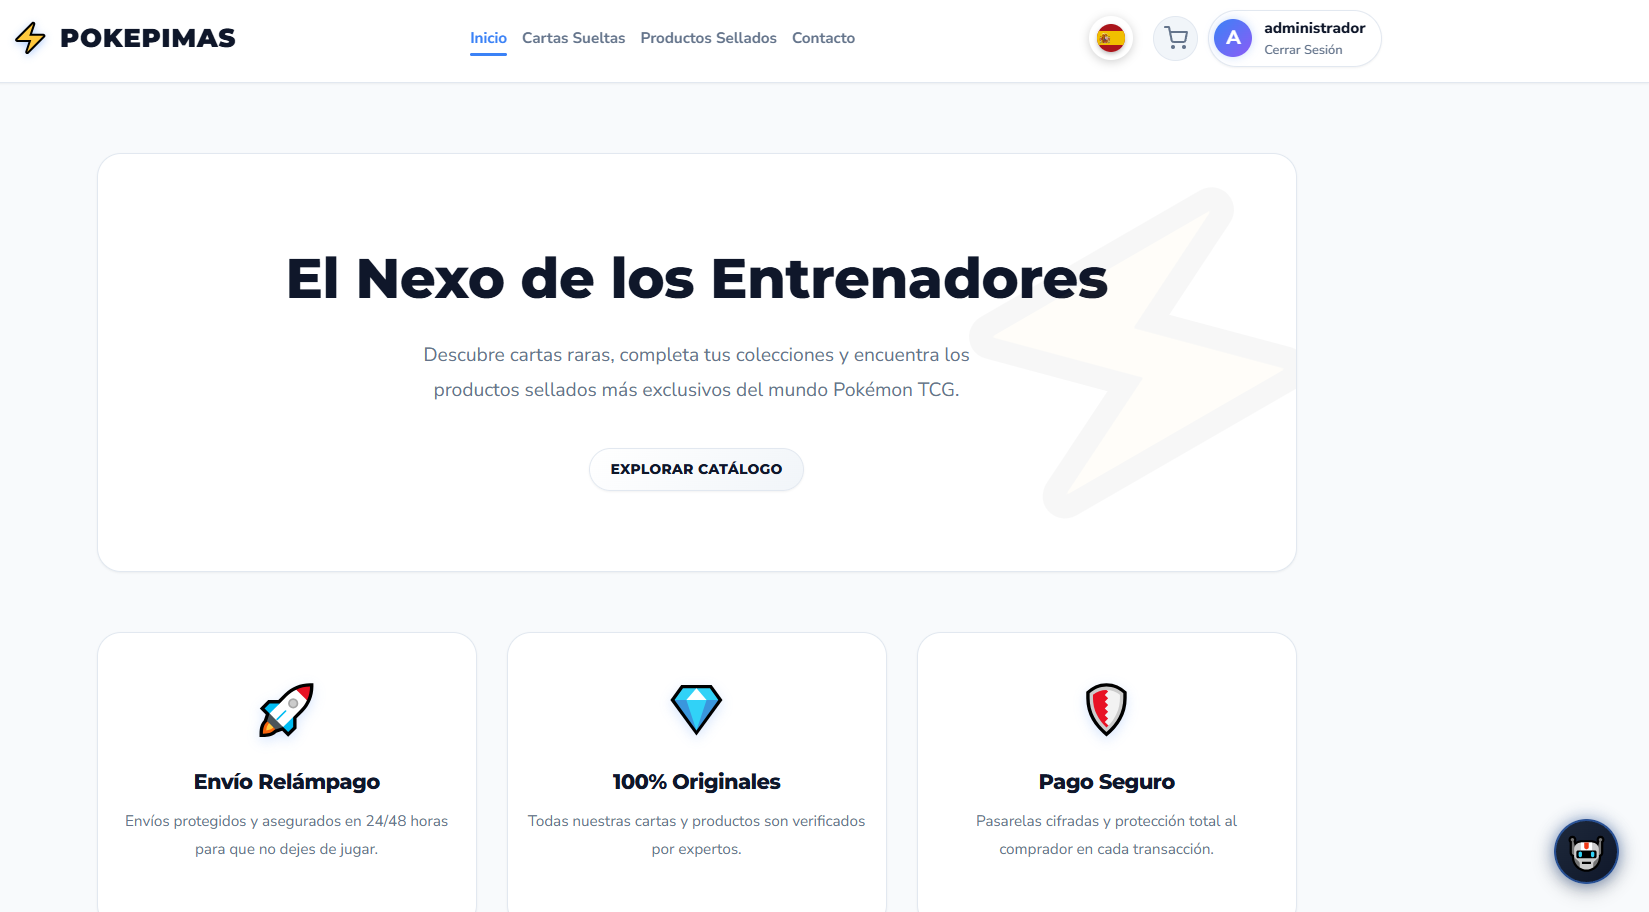
\includegraphics[width=0.8\linewidth]{images/paginaInicio.png}
    \caption{Página de inicio de la tienda web.}
\end{figure}

\begin{figure}[H]
    \centering
    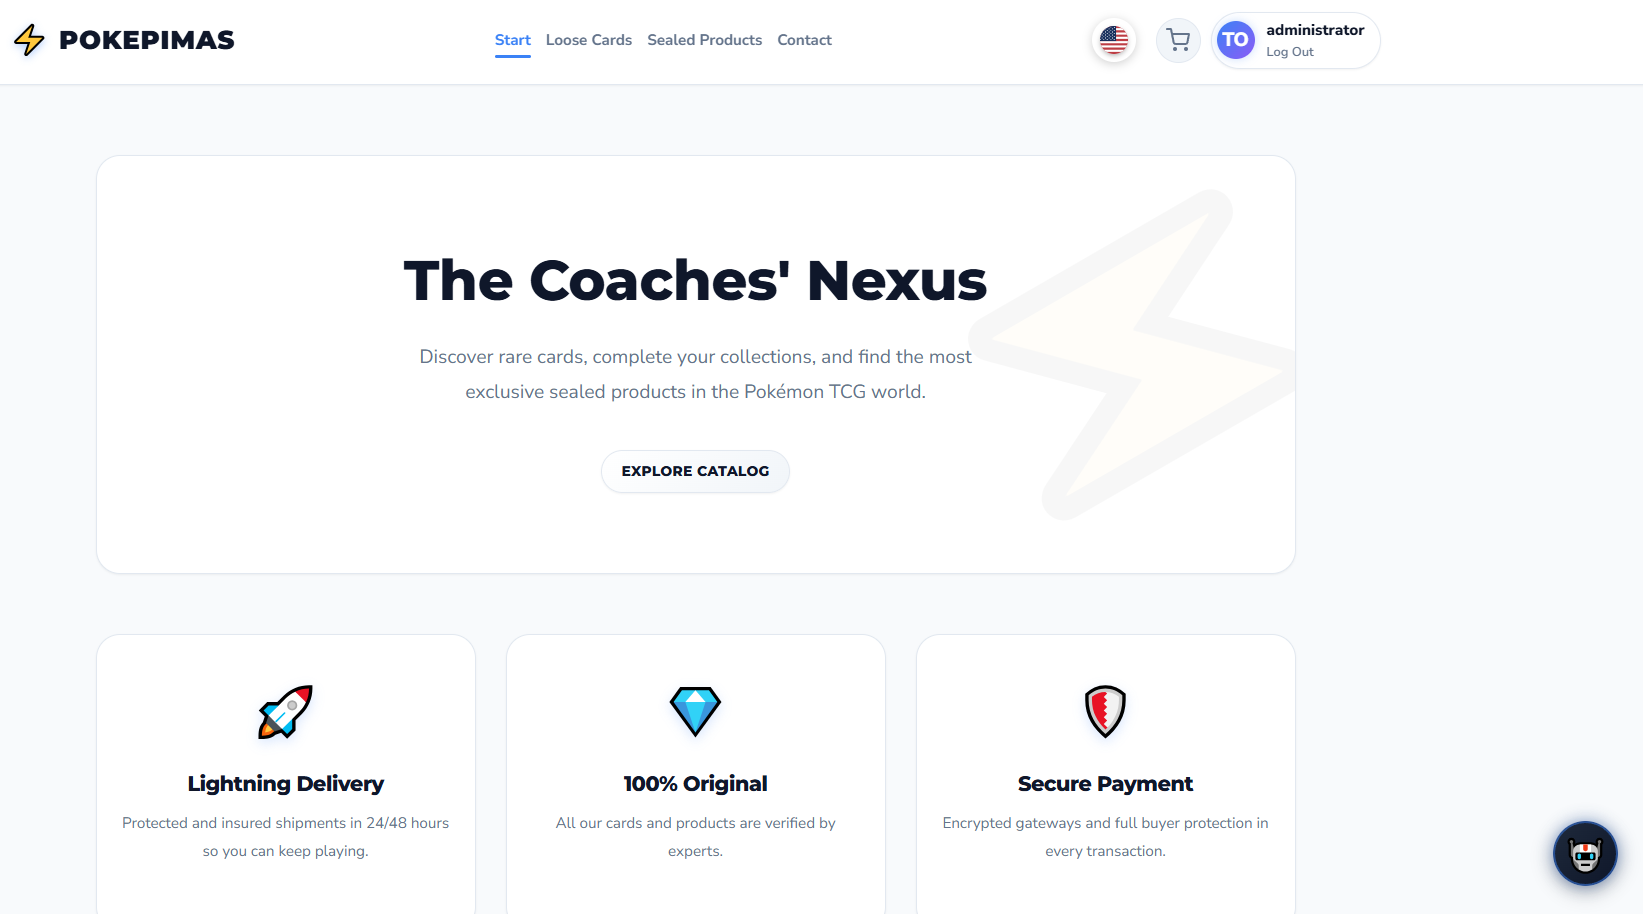
\includegraphics[width=0.8\linewidth]{images/inicioIngles.png}
    \caption{Página de inicio traducida al inglés mediante las banderas.}
\end{figure}

\subsection{Proceso de Compra}
\begin{figure}[H]
    \centering
    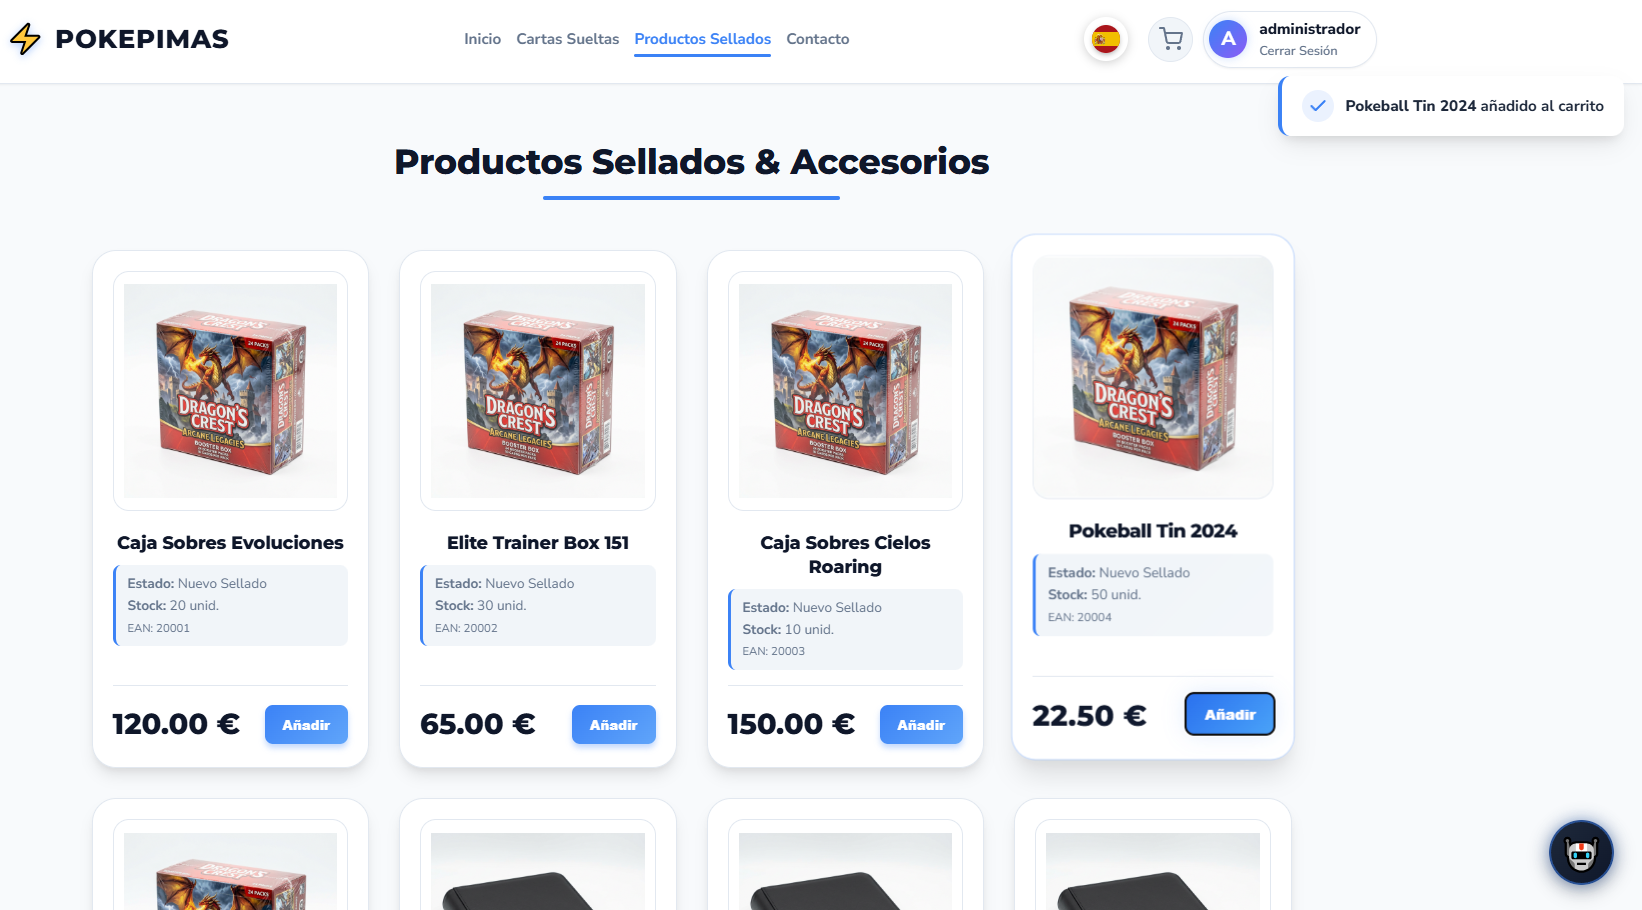
\includegraphics[width=0.8\linewidth]{images/productosSellados+añadirArticulo.png}
    \caption{Vista de productos sellados al añadir un artículo al carrito.}
\end{figure}

\begin{figure}[H]
    \centering
    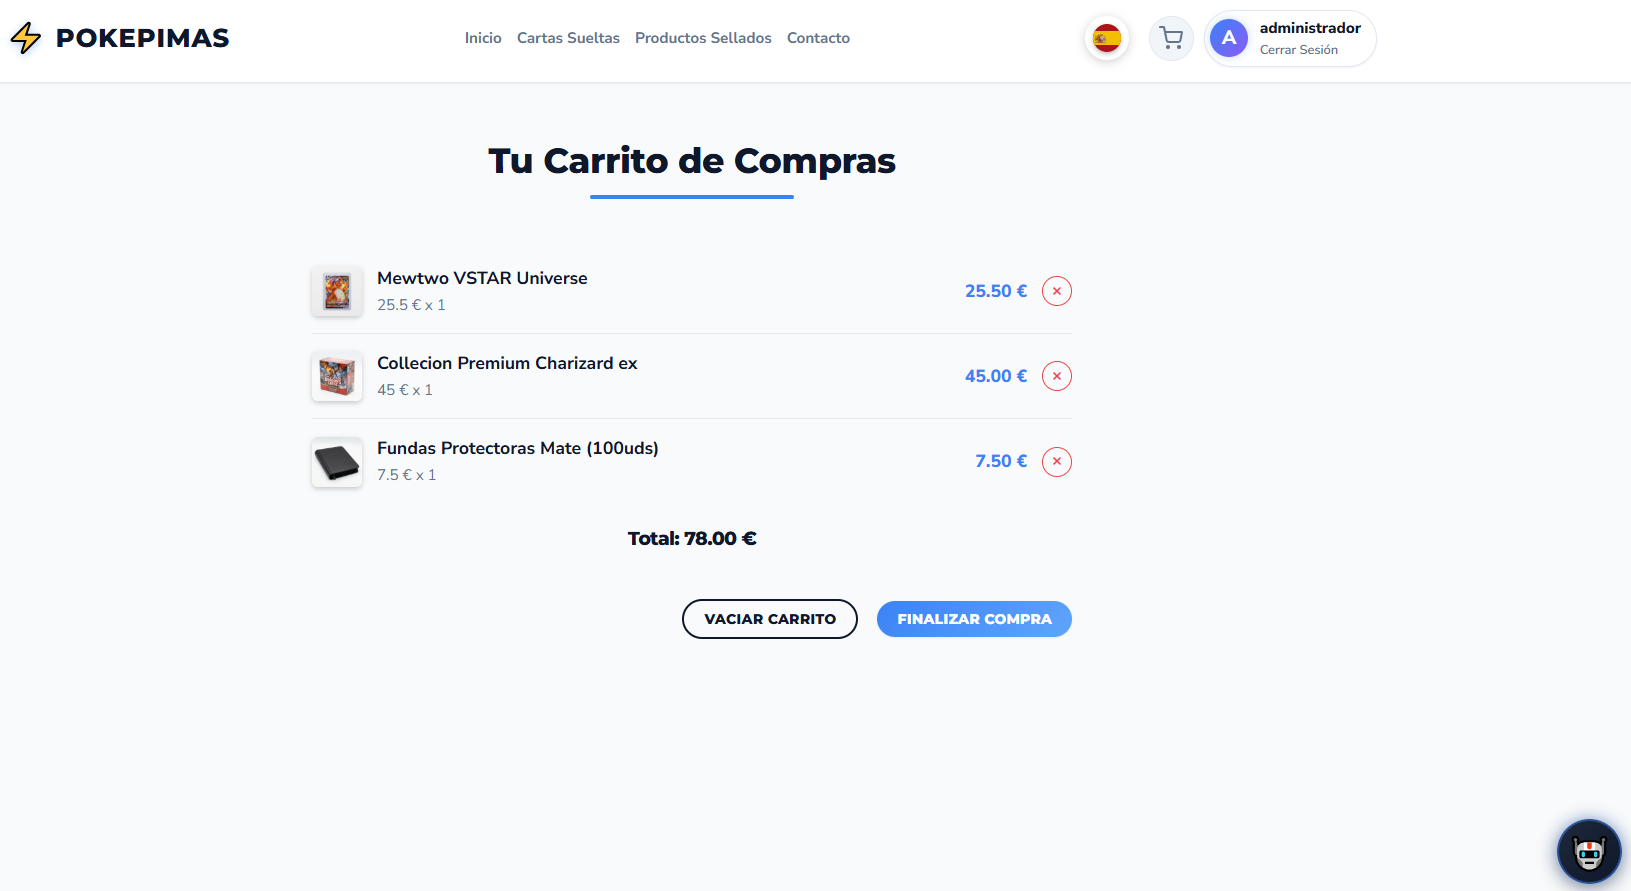
\includegraphics[width=0.8\linewidth]{images/carrito.png}
    \caption{Carrito de compra con los productos añadidos.}
\end{figure}

\subsection{Verificación y Acceso}
\begin{figure}[H]
    \centering
    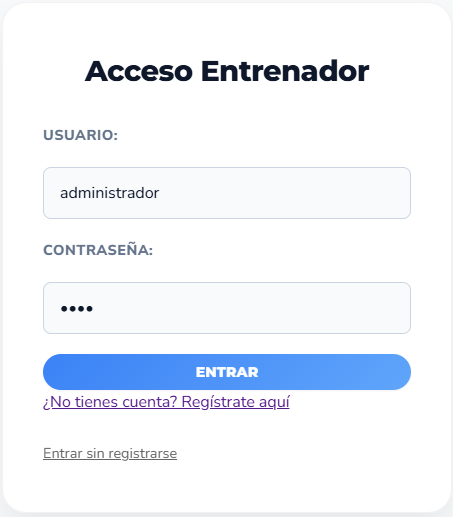
\includegraphics[width=0.8\linewidth]{images/accesoLogin.png}
    \caption{Página de login con un inicio de sesión básico.}
\end{figure}

\subsection{Vista Móvil (Diseño Responsive)}
\begin{figure}[H]
    \centering
    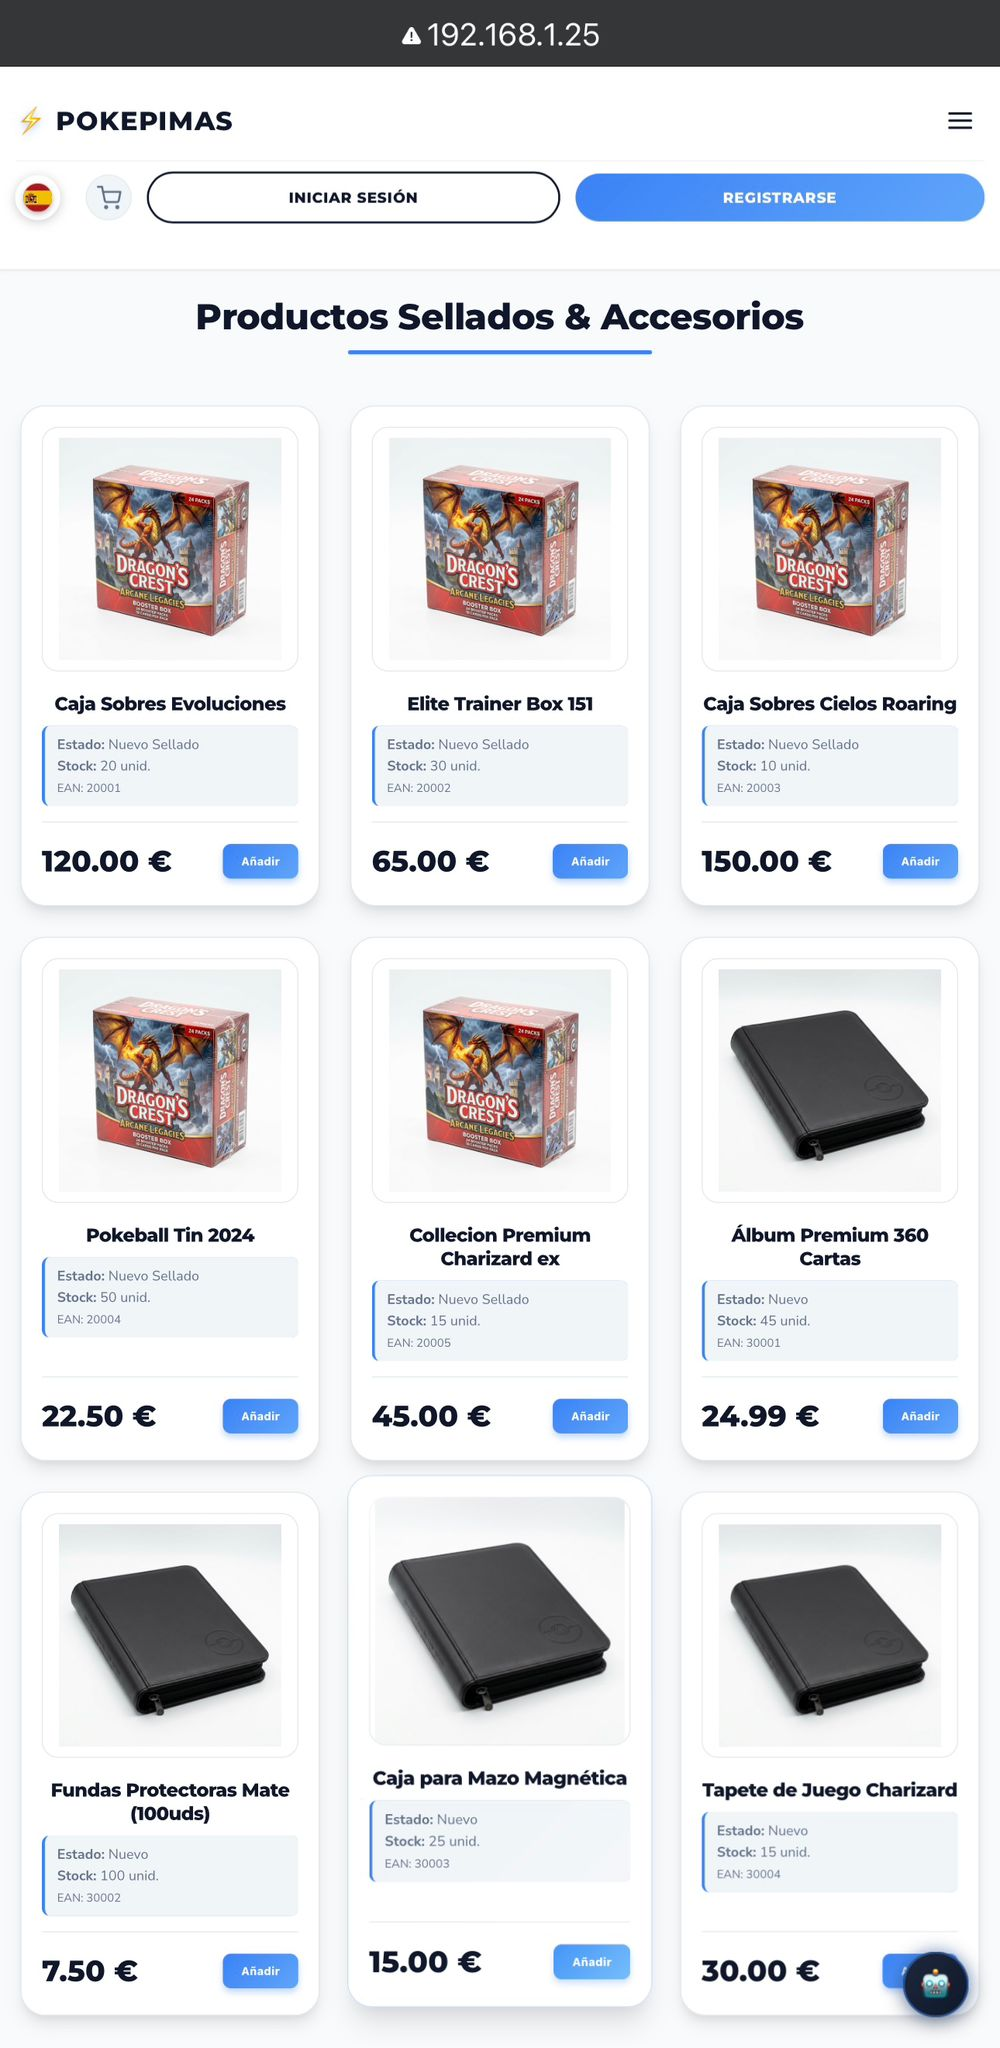
\includegraphics[width=0.45\linewidth]{images/movil1.jpeg}
    \caption{Visualización general adaptada a móvil.}
\end{figure}

\end{document}